\documentclass[a4paper, top=10mm]{article}
%for writing from the top
\usepackage{fullpage}
%for math
\usepackage{amsmath}
\usepackage{mathrsfs}
\usepackage{amsthm}
%for images
\usepackage{graphicx}
\usepackage{tikz}
%for color
\usepackage{xcolor}
%for title
\title{\textbf{\huge{Correct Christmas Tree}}}
\author{Enigma n\textsuperscript{o}5}
\date{14\textsuperscript{th} December 2023}

\newtheorem*{hint}{Hint}

\addtolength{\voffset}{-2cm}
\addtolength{\textheight}{5cm}


\begin{document}
	\maketitle
	
	[statement...]
	
	\begin{center}
		\includegraphics[height=200pt]{00example.png}\\
		Legend
	\end{center}
	
	\begin{center}
		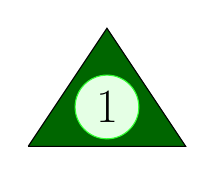
\begin{tikzpicture}
			\filldraw[fill=black!30!green, fill=black!60!green] (0,0.5) -- (1,2) -- (2,0.5) -- (0,0.5);
			\tikzstyle{every node}=[circle,font=\LARGE,draw=green!80,fill=green!10]
			\node at (1,1) {1};
		\end{tikzpicture}
		
		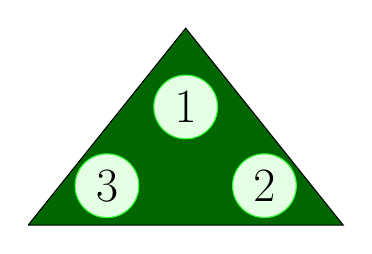
\begin{tikzpicture}
			\filldraw[fill=black!30!green, fill=black!60!green] (-1,-0.5) -- (1,2) -- (3,-0.5) -- (-1,-0.5);
			\tikzstyle{every node}=[circle,font=\LARGE,draw=green!80,fill=green!10]
			\node at (1,1) {1};
			\node at (2,0) {2};
			\node at (0,0) {3};
		\end{tikzpicture}
	\end{center}
	
	
	[question...]
	
\end{document}